% !TEX program = xelatex
% Текст синхронизирован с content.md; оформление основано на timcw.cls Калитвина В.А.
\documentclass{timcw}
\usepackage{longtable,array}
\usepackage{xurl}
\usepackage[hidelinks,unicode]{hyperref}
\setlength{\emergencystretch}{3em}
\titlespacing*{\chapter}{0pt}{0pt}{1.1\baselineskip}
\setlength{\parindent}{1.25cm}
\setlength{\tabcolsep}{4pt}
\renewcommand{\arraystretch}{1.18}
\cwtopic{Разработка клиент-серверного приложения для управления заявками на обслуживание оборудования}
\cwcourse{2}
\cwgroup{ДЭ 21-25}
\cwstudent{Павленко Богдан Евгеньевич}
\cwcityyear{Москва 2026}
\cwdirection{09.03.02 Информационные системы и технологии}
\cwprofile{Большие данные и машинное обучение}
\begin{document}
\cwtitle
{\singlespacing\setlength{\cftbeforetoctitleskip}{0pt}\tableofcontents\par}
\clearpage

\intro

Работа с оборудованием включает не только устранение неисправности, но и передачу информации между людьми. Сотрудник сообщает о проблеме, диспетчер определяет приоритет и назначает исполнителя, техник проводит работы, а ответственный сотрудник принимает результат. Если эти действия обсуждаются только в мессенджере, текущее состояние заявки приходится восстанавливать по сообщениям. Запись «сделано» сама по себе не показывает, кто выполнил работу, что именно изменилось и был ли результат проверен.

В курсовом проекте рассматривается учебная модель службы обслуживания оборудования небольшого учебного подразделения. Диспетчер работает за персональным компьютером, а техник использует телефон непосредственно возле оборудования. Это выбранный сценарий проектирования, а не описание обследованного предприятия. Данные об объектах, сотрудниках и неисправностях являются демонстрационными; внедрение в реальной организации и экономический эффект не заявляются.

Цель работы — разработать клиент-серверное приложение «Контур», обеспечивающее согласованную обработку заявок на обслуживание оборудования на двух устройствах с разграничением полномочий диспетчера и техника.

Для достижения цели необходимо решить следующие задачи:

\begin{itemize}
\item определить участников процесса, границы автоматизации и требования к заявке;
\item спроектировать жизненный цикл заявки, структуру базы данных и программный интерфейс;
\item реализовать серверную проверку прав, сохранение данных и регистрацию событий;
\item разработать интерфейсы диспетчера и техника, пригодные для разных размеров экрана;
\item обеспечить обработку конфликтов при одновременном редактировании;
\item подготовить проверяемые сценарии тестирования и демонстрации на двух устройствах;
\item описать запуск, ограничения и направления дальнейшего развития приложения.
\end{itemize}

Объект исследования — процесс обработки заявок на техническое обслуживание. Предмет исследования — программные средства согласования действий диспетчера и исполнителя в общей информационной системе. Используются методы анализа требований, реляционного моделирования, моделирования состояний, разделения прав и функционального тестирования.

Практическим результатом является приложение с сервером на Python, базой SQLite и адаптивным браузерным интерфейсом. На компьютере и телефоне открываются разные пользовательские сеансы одного сервиса. Такой вариант трактует требование «для двух устройств» как совместную работу двух клиентов с общими данными. Отдельные нативные установочные пакеты для настольной и мобильной операционных систем в область реализации не входят.

Работа состоит из четырёх глав. Первая описывает задачу и требования, вторая — проектные решения, третья — реализацию и пользовательские сценарии, четвёртая — проверку и условия эксплуатации. Оформление пояснительной записки основано на шаблоне, опубликованном преподавателем \cite{src1}.

\chapter{Анализ задачи и формирование требований}

\section{Предметная область и границы проекта}

Заявка в рассматриваемом процессе связывает конкретное оборудование, описание проблемы и ответственного исполнителя. Для небольшого подразделения существенно не количество полей, а однозначность их значения. Например, «высокий приоритет» должен характеризовать срочность обработки, тогда как «в работе» — уже начатое исполнение. Смешение этих понятий делает отчётность неоднозначной: критичная заявка может ещё не иметь исполнителя, а обычная — уже выполняться.

Система разделяет состояние работы и приоритет. Приоритет выбирает диспетчер из четырёх значений: низкий, обычный, высокий и критический. Он не рассчитывается автоматически и не является обещанием времени ремонта. Для расчёта сроков потребовались бы утверждённые регламенты, рабочие календари, категории оборудования и нормативы обслуживания. Таких исходных данных в задании нет, поэтому приложение не изображает несуществующий контроль соглашений об уровне обслуживания.

Основной объект учёта — заявка. Справочник оборудования необходим для выбора объекта без повторного ввода названия и места расположения. Справочник пользователей определяет автора действий и доступные роли. Журнал событий позволяет восстановить последовательность изменений. В область проекта не включены складской учёт запасных частей, закупки, бухгалтерские документы и диспетчеризация выездного транспорта: эти задачи имеют собственные сущности и существенно увеличили бы объём работы.

Пользовательские роли не заменяют должностную структуру предприятия. Роль диспетчера объединяет регистрацию заявки, назначение исполнителя и приёмку результата. Роль техника отвечает за начало и завершение назначенных ему работ. Такое упрощение делает учебный процесс обозримым, сохраняя реальное разделение ответственности: сообщение исполнителя о завершении ещё не означает принятие результата заказчиком.

\section{Сравнение возможных подходов}

На этапе проектирования рассмотрены три способа организации учёта: общая таблица, универсальная доска задач и специализированное приложение. Сравнение является аналитическим: оно отражает особенности подходов, а не результаты испытаний конкретных коммерческих продуктов.

\begingroup\small\singlespacing
\begin{longtable}{>{\raggedright\arraybackslash}p{0.22\textwidth}>{\raggedright\arraybackslash}p{0.22\textwidth}>{\raggedright\arraybackslash}p{0.22\textwidth}>{\raggedright\arraybackslash}p{0.22\textwidth}}
\caption{Сравнение способов учёта заявок}\\
\hline
\textbf{Критерий} & \textbf{Общая таблица} & \textbf{Универсальная доска} & \textbf{Приложение «Контур»} \\ \hline
\endfirsthead
\textbf{Критерий} & \textbf{Общая таблица} & \textbf{Универсальная доска} & \textbf{Приложение «Контур»} \\ \hline
\endhead
Первоначальный запуск & Обычно прост & Требует настройки & Требует установки сервера \\ \hline
Поля оборудования & Настраиваются вручную & Зависят от настроек & Связаны со справочником \\ \hline
Правила переходов & Обычно процедурные & Зависят от продукта & Проверяются сервером \\ \hline
Разделение полномочий & Зависит от доступа к таблице & Зависит от возможностей & Две заданные роли \\ \hline
Объяснимость реализации & Правила задаёт автор таблицы & Правила задаются настройками & Исходный код проекта открыт для проверки \\ \hline
Сопровождение & Необходимо поддерживать структуру & Зависит от сервиса & Ответственность владельца сервера \\ \hline
\end{longtable}
\endgroup

Таблица может быть достаточной для редких обращений и одного ответственного сотрудника. Однако при совместной работе важно ограничивать не только доступ к документу целиком, но и конкретные операции. Технику требуется завершить свою работу, но не назначить другого исполнителя или принять собственный результат от имени диспетчера. Это правило должно быть частью приложения, а не только устной договорённостью.

Универсальная доска задач способна решить значительную часть организационных задач. Самостоятельная разработка не обосновывается утверждением, что готовые системы хуже. Её основание в данном проекте — образовательная цель: построить и объяснить серверный процесс, структуру данных, проверки прав и согласование клиентов. За счёт узкой предметной области можно подробно реализовать один законченный процесс вместо большого количества поверхностных возможностей.

Из сравнения следует выбор небольшого специализированного приложения. Оно не претендует на замену промышленной системы управления обслуживанием. Критерий достаточности — воспроизводимый цикл «создание — назначение — выполнение — приёмка» с сохранением истории и корректной реакцией на ошибочные действия.

\section{Функциональные требования}

Требования сформулированы через наблюдаемое поведение. Это позволяет проверить их независимо от внутренней организации кода. Основные требования приведены в таблице.

\begingroup\small\singlespacing
\renewcommand{\arraystretch}{1.11}
\begin{longtable}{>{\raggedright\arraybackslash}p{0.17\textwidth}>{\raggedright\arraybackslash}p{0.39\textwidth}>{\raggedright\arraybackslash}p{0.35\textwidth}}
\caption{Функциональные требования и критерии проверки}\\
\hline
\textbf{Код} & \textbf{Требование} & \textbf{Признак выполнения} \\ \hline
\endfirsthead
\textbf{Код} & \textbf{Требование} & \textbf{Признак выполнения} \\ \hline
\endhead
ФТ-01 & Вход по учётной записи & Неавторизованный клиент не получает заявки \\ \hline
ФТ-02 & Создание заявки диспетчером & Сохранены оборудование, заголовок, описание и приоритет \\ \hline
ФТ-03 & Назначение техника & Заявка появляется в списке назначенного исполнителя \\ \hline
ФТ-04 & Начало выполнения & Назначенный техник переводит заявку в работу \\ \hline
ФТ-05 & Завершение с результатом & Пустое описание результата отклоняется \\ \hline
ФТ-06 & Приёмка диспетчером & Выполненная заявка становится закрытой \\ \hline
ФТ-07 & Возврат на доработку & Выполненная или закрытая заявка снова назначена \\ \hline
ФТ-08 & История и комментарии & Видны автор, время и содержание события \\ \hline
ФТ-09 & Поиск и фильтрация & Пользователь сужает список без изменения данных \\ \hline
ФТ-10 & Экспорт диспетчером & Создаётся CSV с доступными диспетчеру заявками \\ \hline
ФТ-11 & Совместная работа & Второй сеанс получает сохранённые изменения \\ \hline
ФТ-12 & Контроль версии & Устаревшее изменение отклоняется как конфликт \\ \hline
\end{longtable}
\endgroup

Назначение разрешено только до начала выполнения. Иначе простой выбор нового имени мог бы скрыто передать уже выполняемую работу другому человеку. Для более сложного перевода между исполнителями потребовались бы отдельные причина, подтверждение и правила ответственности. В текущем проекте такое действие намеренно отсутствует.

Комментарий и изменение состояния имеют разный смысл. Комментарий уточняет обстоятельства, но не заменяет переход статуса. Фраза «всё готово» в комментарии не должна закрывать заявку. Поэтому завершение выполняется отдельной операцией с обязательным описанием результата, а комментарии остаются независимыми событиями обсуждения.

\section{Нефункциональные требования и критерии качества}

Согласованность данных важнее мгновенной анимации интерфейса. Сервер должен проверять права и допустимость переходов даже при прямом запросе к API. Отсутствие кнопки на экране не является защитой: клиентский код выполняется на устройстве пользователя и может быть изменён. Именно сервер определяет, какое действие допустимо для текущей учётной записи.

Приложение должно сохранять заявки после перезапуска, не требовать внешних облачных сервисов для основного сценария и работать в браузерах компьютера и телефона. Исходные файлы интерфейса обслуживаются тем же сервером, что и API. Внешние шрифты, библиотеки и системы аналитики не требуются для отображения страницы, что упрощает демонстрацию в локальной сети.

Критерии удобства включают читаемые подписи, различение приоритета и состояния не только цветом, возможность закрыть диалог с клавиатуры и отсутствие горизонтальной прокрутки основного интерфейса на узком экране. Ошибка сервера должна приводить к понятному сообщению, а не к исчезновению введённого текста. Сетевой сбой не должен отображаться как успешное сохранение.

\looseness=-1 Система проектируется для учебной демонстрации небольшой рабочей группы. Измеренные пределы производительности и число одновременно обслуживаемых пользователей не заявляются. Для промышленной эксплуатации потребовались бы нагрузочные испытания, политика резервного копирования, мониторинг и развёртывание с HTTPS. Эти условия отделены от функциональной готовности учебного приложения.

\chapter{Проектирование приложения}

\section{Архитектура и выбор технологий}

Приложение построено по клиент-серверной архитектуре. Клиент отвечает за представление данных, ввод и отображение ошибок; сервер — за аутентификацию, правила работы и обращения к базе. SQLite хранит пользователей, оборудование, заявки и события. Оба устройства взаимодействуют с одним сервером, поэтому на телефоне не создаётся отдельная копия производственной базы.

Выбран Python с Flask. Flask предоставляет маршрутизацию HTTP-запросов, обработку запросов и механизм сеансов; предметные правила реализуются явно в коде приложения \cite{src2}. Это позволяет проследить полный путь операции без большого числа вспомогательных компонентов. Сервер Waitress используется для обслуживания WSGI-приложения; он работает в одном процессе с несколькими потоками и подходит для выбранного способа запуска \cite{src3}.

SQLite выбрана потому, что учебному проекту требуется постоянное реляционное хранилище, но не отдельная служба администрирования СУБД. Работа с файлом базы снижает число шагов установки. При этом SQLite допускает только одного одновременно выполняющего запись участника транзакции; данное ограничение необходимо учитывать при росте нагрузки \cite{src4}. Выбор не означает, что файловая база подходит для любого масштаба.

Клиент реализован на HTML, CSS и JavaScript без системы сборки. Асинхронные HTTP-запросы выполняются через Fetch API. Сам факт получения ответа не означает успех прикладной операции: интерфейс проверяет HTTP-статус и обрабатывает ошибочный ответ отдельно \cite{src7}. Адаптация к размерам экрана осуществляется средствами CSS, включая медиазапросы \cite{src9}.

Взаимодействие начинается с загрузки страницы и получения текущего сеанса. После входа клиент получает справочные данные и список доступных заявок. Диспетчеру показывается общая очередь, технику — только его задания. Изменения отправляются отдельными запросами. После подтверждения сервером клиент обновляет представление; другие открытые клиенты получают изменения при следующем опросе.

\IfFileExists{architecture.png}{\begin{figure}[htbp]\centering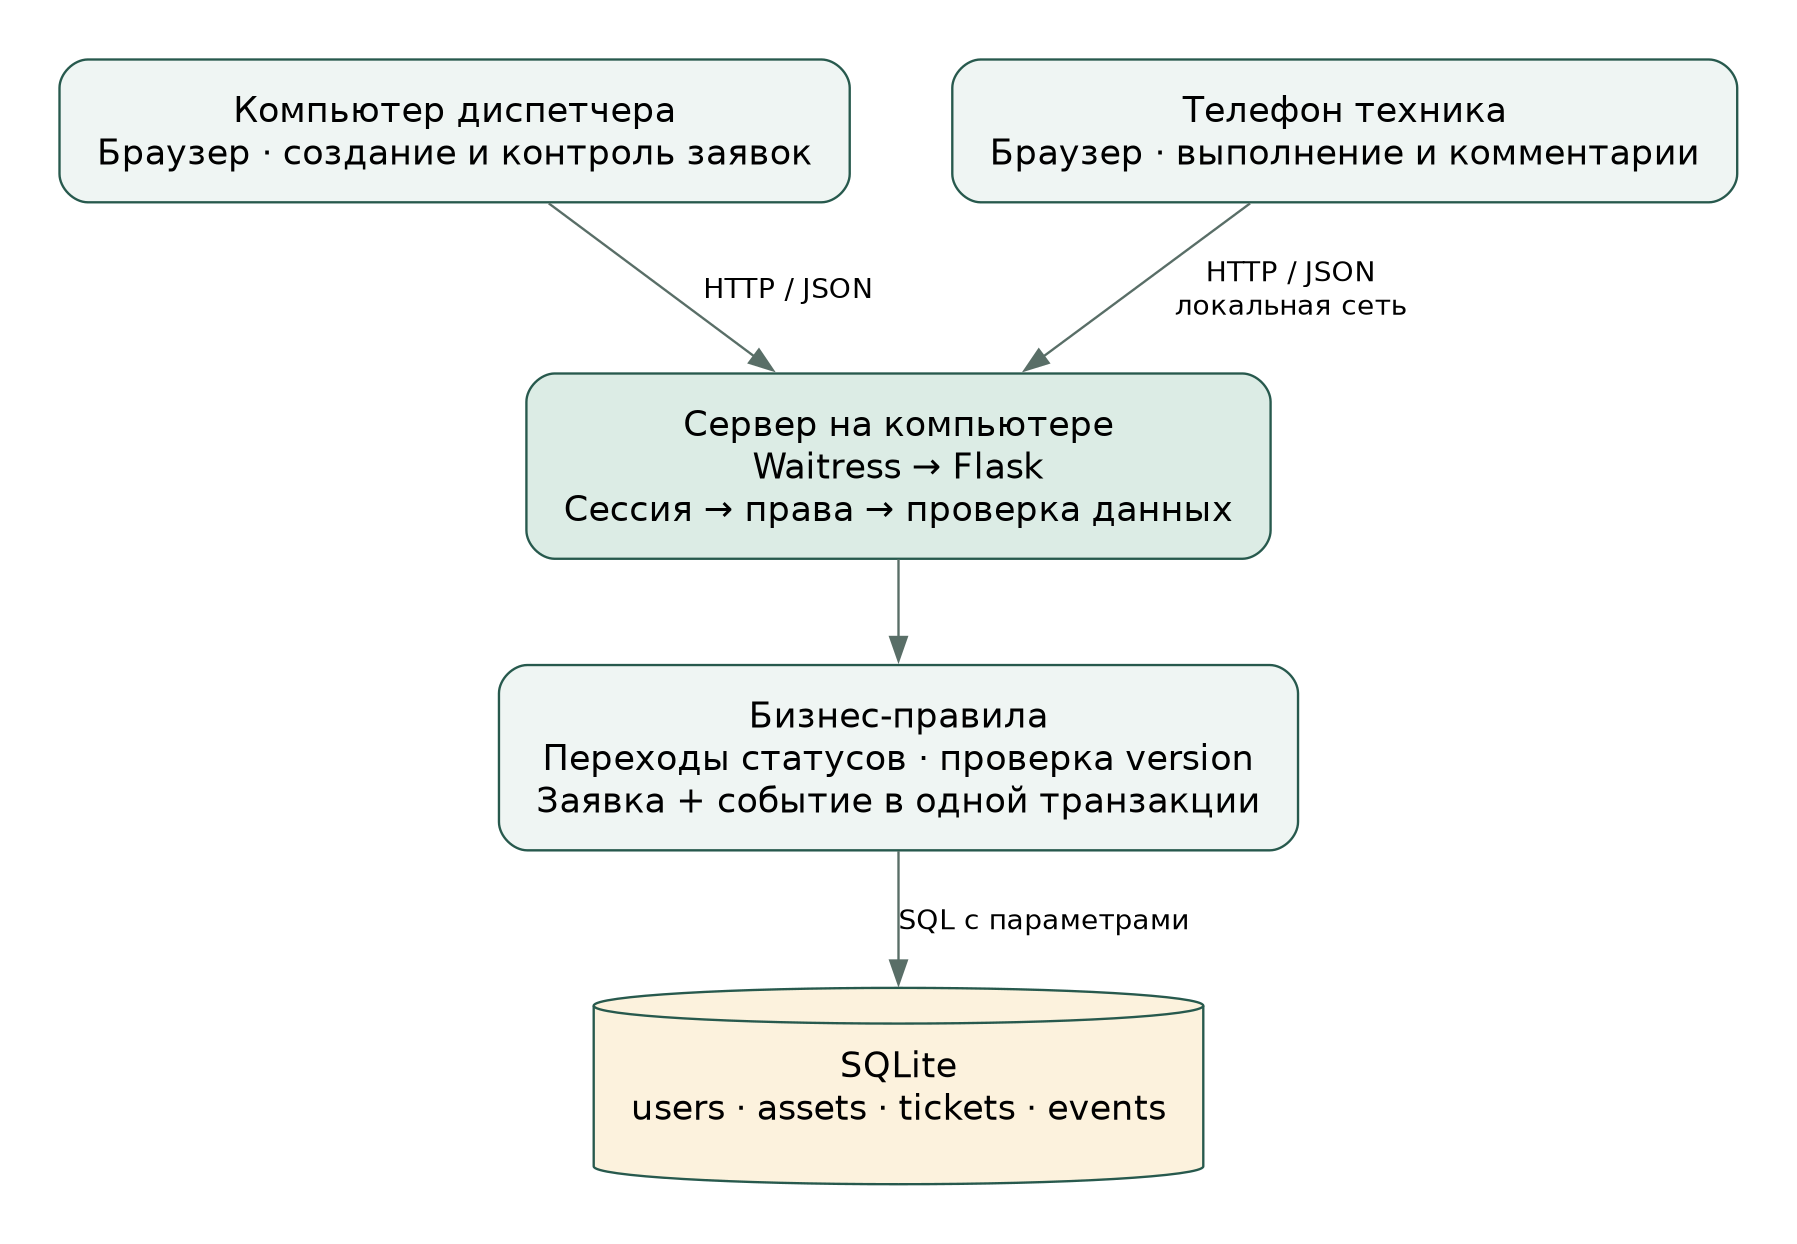
\includegraphics[width=0.96\textwidth]{architecture.png}\caption{Архитектура приложения «Контур»}\end{figure}}{}

Отказ от микросервисов и отдельного фронтенд-фреймворка является сознательным решением. В проекте один основной процесс и одна база. Разделение его на сетевые службы добавило бы вопросы доставки сообщений и согласования распределённых данных, не улучшив выполнение исходного задания. Граница между клиентом и сервером при этом остаётся явно выраженной через API.

\section{Модель данных}

Модель включает четыре основные сущности: пользователь, оборудование, заявка и событие заявки. Пользователь может быть назначен исполнителем многих заявок; оборудование может фигурировать в нескольких обращениях за разные даты; каждая заявка имеет множество событий. Связи позволяют хранить имя оборудования и пользователя один раз, а в заявках использовать идентификаторы.

\begingroup\small\singlespacing
\begin{longtable}{>{\raggedright\arraybackslash}p{0.17\textwidth}>{\raggedright\arraybackslash}p{0.39\textwidth}>{\raggedright\arraybackslash}p{0.35\textwidth}}
\caption{Сущности модели данных}\\
\hline
\textbf{Сущность} & \textbf{Основные сведения} & \textbf{Назначение} \\ \hline
\endfirsthead
\textbf{Сущность} & \textbf{Основные сведения} & \textbf{Назначение} \\ \hline
\endhead
Пользователь & Идентификатор, логин, имя, хеш пароля, роль & Вход и определение полномочий \\ \hline
Оборудование & Идентификатор, название, расположение, инвентарный номер & Однозначный выбор объекта \\ \hline
Заявка & Заголовок, описание, оборудование, приоритет, статус, исполнитель, версия, даты & Текущее состояние работы \\ \hline
Событие & Заявка, автор, тип, текст, время & История изменений и обсуждение \\ \hline
\end{longtable}
\endgroup

Внешние ключи поддерживают ссылочную целостность: заявка не должна ссылаться на отсутствующее оборудование, а событие — на отсутствующую заявку. В SQLite контроль внешних ключей включается для соединения явно \cite{src5}. На уровне приложения также проверяется, что назначаемый пользователь существует и имеет роль техника; одного внешнего ключа для такого предметного ограничения недостаточно.

Версия заявки — положительное целое число, изменяемое при обновлении её рабочих полей. Она не является временем и не вычисляется из часов устройства. Два клиента могут иметь разные локальные часы, но сравнение целых версий остаётся однозначным. Поля времени служат для отображения хронологии; сервер передаёт время в формате ISO с обозначением UTC, а интерфейс представляет его пользователю.

Имена исполнителей и названия оборудования возвращаются в API вместе с идентификаторами, чтобы клиенту не приходилось вручную соединять таблицы. Это представление данных, а не дублирование хранения: сервер получает связанные сведения запросом. Изменение имени пользователя не требует переписывать все его заявки. При этом историческая неизменность отображаемого имени не заявляется: журнал ссылается на автора через идентификатор.

\IfFileExists{schema.png}{\begin{figure}[htbp]\centering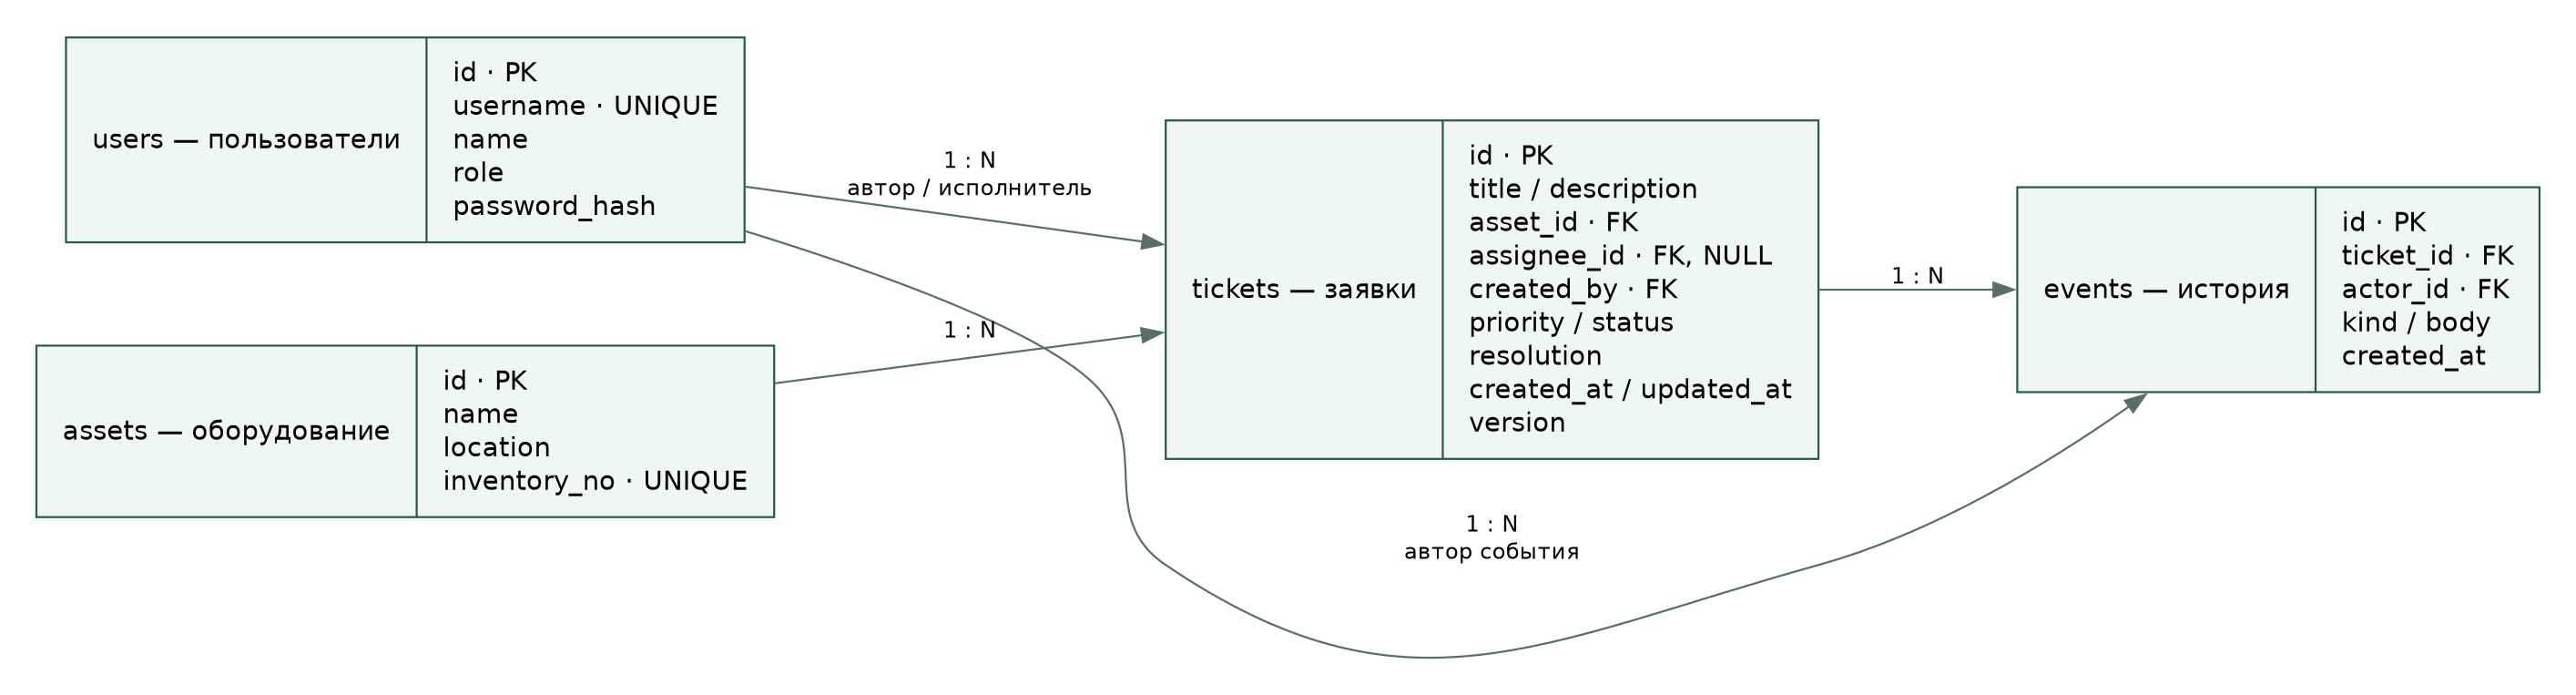
\includegraphics[width=0.96\textwidth]{schema.png}\caption{Основные сущности и связи базы данных}\end{figure}}{}

Разделение текущего состояния и истории решает разные задачи. Для вывода очереди достаточно одной записи заявки. Для ответа на вопрос «почему она снова назначена?» необходимы события. История дополняет состояние, но не используется как единственный источник для его вычисления. Такая схема проще событийной архитектуры и достаточна для проекта.

\section{Жизненный цикл и полномочия}

Жизненный цикл состоит из пяти состояний: новая, назначена, в работе, выполнена и закрыта. Новая заявка зарегистрирована, но ещё не имеет исполнителя. Назначенная заявка ожидает начала работ. Выполненная содержит результат техника, но ещё не принята диспетчером. Закрытие фиксирует завершение организационного процесса.

\begingroup\small\singlespacing
\begin{longtable}{>{\raggedright\arraybackslash}p{0.22\textwidth}>{\raggedright\arraybackslash}p{0.22\textwidth}>{\raggedright\arraybackslash}p{0.22\textwidth}>{\raggedright\arraybackslash}p{0.22\textwidth}}
\caption{Переходы между состояниями заявки}\\
\hline
\textbf{Исходное состояние} & \textbf{Действие} & \textbf{Результат} & \textbf{Кто выполняет} \\ \hline
\endfirsthead
\textbf{Исходное состояние} & \textbf{Действие} & \textbf{Результат} & \textbf{Кто выполняет} \\ \hline
\endhead
Новая & Назначить техника & Назначена & Диспетчер \\ \hline
Назначена & Начать работу & В работе & Назначенный техник \\ \hline
В работе & Указать результат & Выполнена & Назначенный техник \\ \hline
Выполнена & Принять результат & Закрыта & Диспетчер \\ \hline
Выполнена / закрыта & Вернуть на доработку & Назначена & Диспетчер \\ \hline
\end{longtable}
\endgroup

Создание с уже выбранным исполнителем сразу формирует назначенную заявку. Этот путь не пропускает проверку полномочий: исполнитель задаётся диспетчером в момент регистрации. Возврат на доработку сохраняет назначенного техника, чтобы новое действие имело ответственного. Если требуется сменить исполнителя после возврата, диспетчер делает это отдельной операцией в состоянии «назначена».

Для техника проверяются одновременно роль и принадлежность заявки. Недостаточно установить, что пользователь является техником: он не должен получать содержание чужой задачи или менять её статус. Ограничение применяется к списку, карточке, комментариям и изменению заявки. Проверка только в одном из этих мест оставила бы обходной путь через другой маршрут.

Переходы представлены как конечный набор разрешённых действий, а не как свободный выбор любого статуса. Например, переход из «новая» сразу в «закрыта» не допускается. Такой подход поддерживает смысл журнала: каждой важной стадии соответствует реальное действие определённой роли. Сервер повторно проверяет состояние после получения запроса, поскольку открытая карточка могла устареть.

\section{Программный интерфейс}

API передаёт данные в формате JSON. Идентификаторы являются числами, значения статуса и приоритета — фиксированными строками. Это уменьшает неоднозначность: слово «срочная» из произвольного текста не может случайно стать новым допустимым приоритетом. Проверяются наличие обязательных полей, типы, длины текста и существование связанных объектов.

\begingroup\small\singlespacing
\begin{longtable}{>{\raggedright\arraybackslash}p{0.34\textwidth}>{\raggedright\arraybackslash}p{0.58\textwidth}}
\caption{Операции программного интерфейса}\\
\hline
\textbf{Метод и путь} & \textbf{Смысл} \\ \hline
\endfirsthead
\textbf{Метод и путь} & \textbf{Смысл} \\ \hline
\endhead
GET /api/session & Текущий пользователь и CSRF-токен \\ \hline
POST /api/login & Проверка учётных данных \\ \hline
POST /api/logout & Завершение сеанса \\ \hline
GET /api/meta & Доступные справочники \\ \hline
GET /api/tickets & Список заявок с учётом роли \\ \hline
POST /api/tickets & Создание диспетчером \\ \hline
GET /api/tickets/\{id\} & Карточка и события \\ \hline
PATCH /api/tickets/\{id\} & Изменение с проверкой версии \\ \hline
POST /api/tickets/\{id\}/comments & Добавление комментария \\ \hline
GET /api/export.csv & Выгрузка для диспетчера \\ \hline
\end{longtable}
\endgroup

Успех операции возвращается только после сохранения данных. Ошибки представлены структурированным объектом с понятным описанием. Для конфликта версии применяется HTTP 409: этот статус сообщает о противоречии между запросом и текущим состоянием ресурса \cite{src8}. Ошибки ввода, отсутствие авторизации и запрет операции разделяются, чтобы интерфейс мог показать правильную причину.

Запрос изменения содержит номер версии, которую видел пользователь. Номер заявки передаётся в адресе, а изменяемые поля — в теле. Сервер не доверяет присланной роли пользователя или имени автора: эти сведения определяются по сеансу. Аналогично время события формируется сервером, а не берётся из пользовательского текста.

\section{Обработка одновременных изменений}

Общая база данных сама по себе не устраняет потерянные обновления. Пусть диспетчер открыл заявку версии 3, затем техник перевёл её в работу, сформировав версию 4. Если диспетчер сохранит старую форму без проверки, его изменения могут опираться на уже неверное состояние. Особенно опасна передача полного старого объекта: вместе с изменённым полем могут вернуться устаревшие значения остальных полей.

В «Контуре» применяется оптимистический контроль: клиент присылает ожидаемую версию, а сервер обновляет запись только при совпадении. Условие имеет смысл «изменить заявку с этим идентификатором, если её версия по-прежнему равна ожидаемой». Успешная операция увеличивает версию. Если подходящая запись не обновлена, запрос завершается конфликтом, а клиент должен получить актуальные данные и повторить осознанное действие.

Проверка и изменение должны образовывать одну согласованную операцию. Простая последовательность «прочитать версию — сравнить — безусловно записать» недостаточна: между сравнением и записью может вмешаться другой запрос. Поэтому существенны условие версии непосредственно в SQL-обновлении и транзакция. Изменение заявки и запись связанного события фиксируются вместе; при ошибке нельзя оставить обновлённый статус без истории.

Комментарии добавляются как новые события и не перезаписывают текст предыдущего комментария. Поэтому конфликт двух комментариев не требует выбора победителя: оба могут сохраниться. Это отличается от изменения единственного поля приоритета. Контроль версии используется там, где обновляется текущее состояние заявки, а не механически для каждой записи в системе.

\chapter{Реализация и работа пользователей}

\section{Организация серверной части}

Сервер создаёт приложение, подключает обработчики маршрутов и открывает соединения с SQLite для выполнения запросов. SQL-параметры передаются отдельно от текста запроса. Модуль sqlite3 поддерживает параметризованное выполнение; значения пользователя не требуется вставлять в SQL путём склеивания строк \cite{src6}. Это одновременно упрощает обработку кавычек и устраняет соответствующий путь SQL-инъекции.

При изменении заявки сервер сначала сверяет токен сеанса и проверяет источник запроса, если браузер передал заголовок Origin. Затем обработчик устанавливает пользователя, проверяет полномочия, поля и допустимость операции. Запись выполняется внутри транзакции. Для операции техника добавляется проверка назначения. Ошибка на раннем этапе прекращает обработку до записи. За счёт этого один и тот же инвариант сохраняется независимо от того, нажал пользователь штатную кнопку или отправил запрос иным клиентом.

Инварианты системы можно сформулировать следующим образом: у каждой заявки существует оборудование; назначенный исполнитель является техником; техник видит только собственные задания; выполненная работа содержит описание результата; версия не уменьшается; рабочее изменение сопровождается событием. Эти свойства важнее конкретного расположения функций в файле, поскольку непосредственно определяют корректность поведения.

Для начального знакомства предусмотрена явная команда создания демонстрационных данных. Она добавляет синтетические учётные записи и примеры заявок. Демонстрационные пароли опубликованы для воспроизводимости учебного сценария и не считаются пригодными для реальной эксплуатации. Инициализация демонстрации отделена от обычного запуска: запуск сервера не должен незаметно создавать известные всем учётные записи в рабочей базе.

Перезапуск процесса не очищает базу. Вместе с файлом данных сохраняется секрет подписи сеансов. Секрет и локальная база относятся к эксплуатационным файлам, а не к исходному коду для GitHub. Публикация проекта должна включать программу и инструкцию, но исключать пользовательские данные, ключи, локальное окружение и временные файлы.

\section{Аутентификация и защита операций}

Пароль проверяется по стойкому хешу, а не хранится открытым текстом. Используется готовая функция библиотеки Werkzeug, а не собственная криптографическая конструкция. Общий принцип медленного хеширования паролей и применения соли соответствует рекомендациям OWASP \cite{src11}. Знание демонстрационного пароля из инструкции не раскрывает способ хранения других паролей, но делает соответствующую демонстрационную учётную запись открытой для всех читателей.

Сеанс позволяет связать последующие запросы с прошедшим вход пользователем. Подпись cookie защищает её содержимое от незаметной подмены, но не шифрует данные и не заменяет проверку прав. В cookie не требуется хранить пароль. Параметры cookie ограничивают доступ к ней из JavaScript и поведение при межсайтовых запросах; соответствующие механизмы входят в средства защиты Flask \cite{src12}.

Изменяющие запросы сопровождаются CSRF-токеном. Клиент получает его при запросе сеанса и отправляет в специальном заголовке. Сервер сравнивает токен с ожидаемым. Это защищает от ситуации, когда чужой сайт пытается инициировать действие от имени уже вошедшего пользователя. Использование токена и пользовательского заголовка соответствует подходам, описанным OWASP \cite{src10}. Авторизация всё равно нужна: правильный токен не даёт технику полномочий диспетчера.

Защита вывода также отличается от защиты запросов. Название заявки и комментарий могут содержать символы разметки. Интерфейс должен показывать их как текст, а не исполнять как HTML. Проверка длины не решает эту задачу: даже короткая строка может иметь специальный смысл в браузере. Интерфейс записывает значения в текстовые свойства элементов или экранирует специальные символы перед вставкой в HTML-шаблон.

Для CSV существует отдельная особенность: табличная программа может интерпретировать значение, начинающееся со знака формулы, как выражение. Поэтому экспорт должен экранировать потенциально опасные текстовые значения. Обычные CSV-кавычки обеспечивают структуру файла, но сами по себе не запрещают вычисление формулы при открытии в редакторе таблиц.

Указанные меры не превращают локальный учебный сервер в полностью подготовленный интернет-сервис. При HTTP содержимое запросов не защищено шифрованием канала. Основной сценарий ограничен доверенной локальной сетью с демонстрационными данными. Публичная публикация требует HTTPS, новых паролей, управления учётными записями и отдельной проверки конфигурации.

\section{Интерфейс диспетчера}

После входа диспетчер видит общую очередь и сводные показатели по имеющимся заявкам. Числа рассчитываются по доступным данным, а не являются декоративными значениями. Поиск и фильтры помогают выделить состояние или приоритет. Поскольку список принадлежит рабочему процессу, основное действие — создание заявки — находится рядом с очередью, а не скрывается в настройках.

Форма создания включает заголовок, описание, оборудование, приоритет и необязательного исполнителя. Заголовок кратко обозначает проблему; описание сообщает воспроизводимые обстоятельства. Например, «Принтер не печатает» является заголовком, а «задание остаётся в очереди, индикатор бумаги не горит» — полезным уточнением. Интерфейс не пытается автоматически определять причину неисправности по тексту.

Карточка объединяет текущие поля и хронологию. Диспетчер может назначить техника до начала работ, изменить приоритет и прокомментировать обращение. Когда техник отмечает выполнение, диспетчер читает результат и либо закрывает заявку, либо возвращает её на доработку. Возврат сопровождается обсуждением причины; сам по себе статус не заменяет содержательного пояснения.

Экспорт предназначен для внешнего просмотра очереди и подготовки отчёта. CSV является снимком на момент запроса, а не второй синхронизируемой базой. Изменение экспортированного файла не меняет сервер. Это важно объяснить пользователю, иначе редактирование выгрузки может восприниматься как альтернативный способ управления заявками.

\begin{figure}[htbp]\centering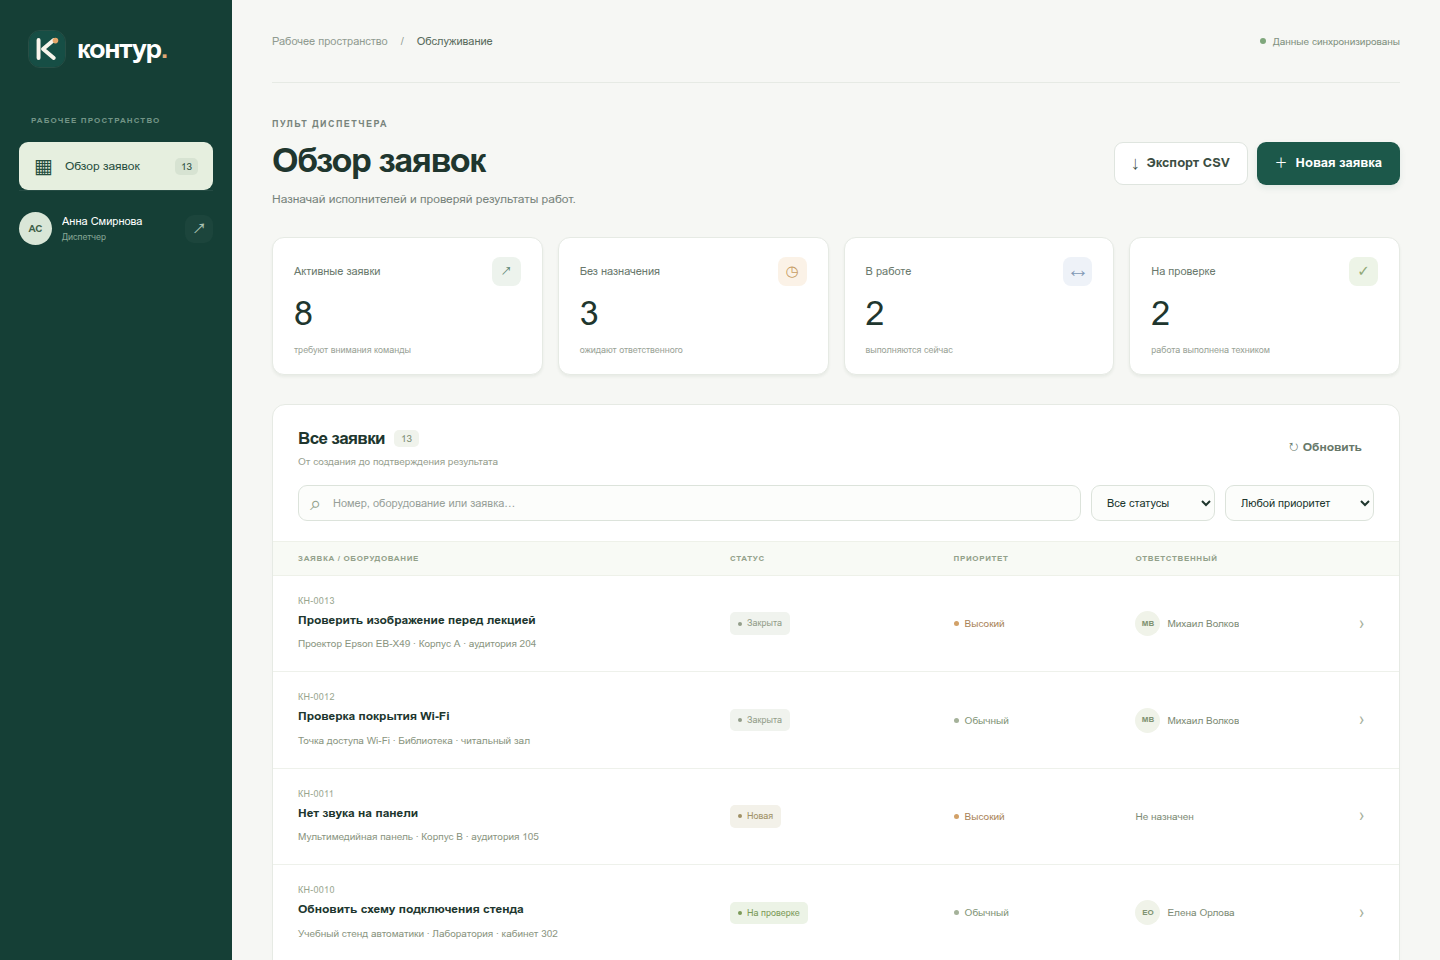
\includegraphics[width=0.99\textwidth,height=0.62\textheight,keepaspectratio]{screens/desktop.png}\caption{Рабочее место диспетчера при регистрации заявки}\end{figure}

\section{Интерфейс техника на телефоне}

Технику требуется быстро увидеть свою следующую работу, место расположения оборудования и описание проблемы. Поэтому мобильное представление ориентировано на карточки и основные действия, а не на широкую таблицу. Пользователь не должен уменьшать страницу пальцами, чтобы нажать кнопку начала работы. Приоритет и состояние имеют текстовые подписи и не зависят исключительно от цветового различения.

\begin{figure}[!ht]\centering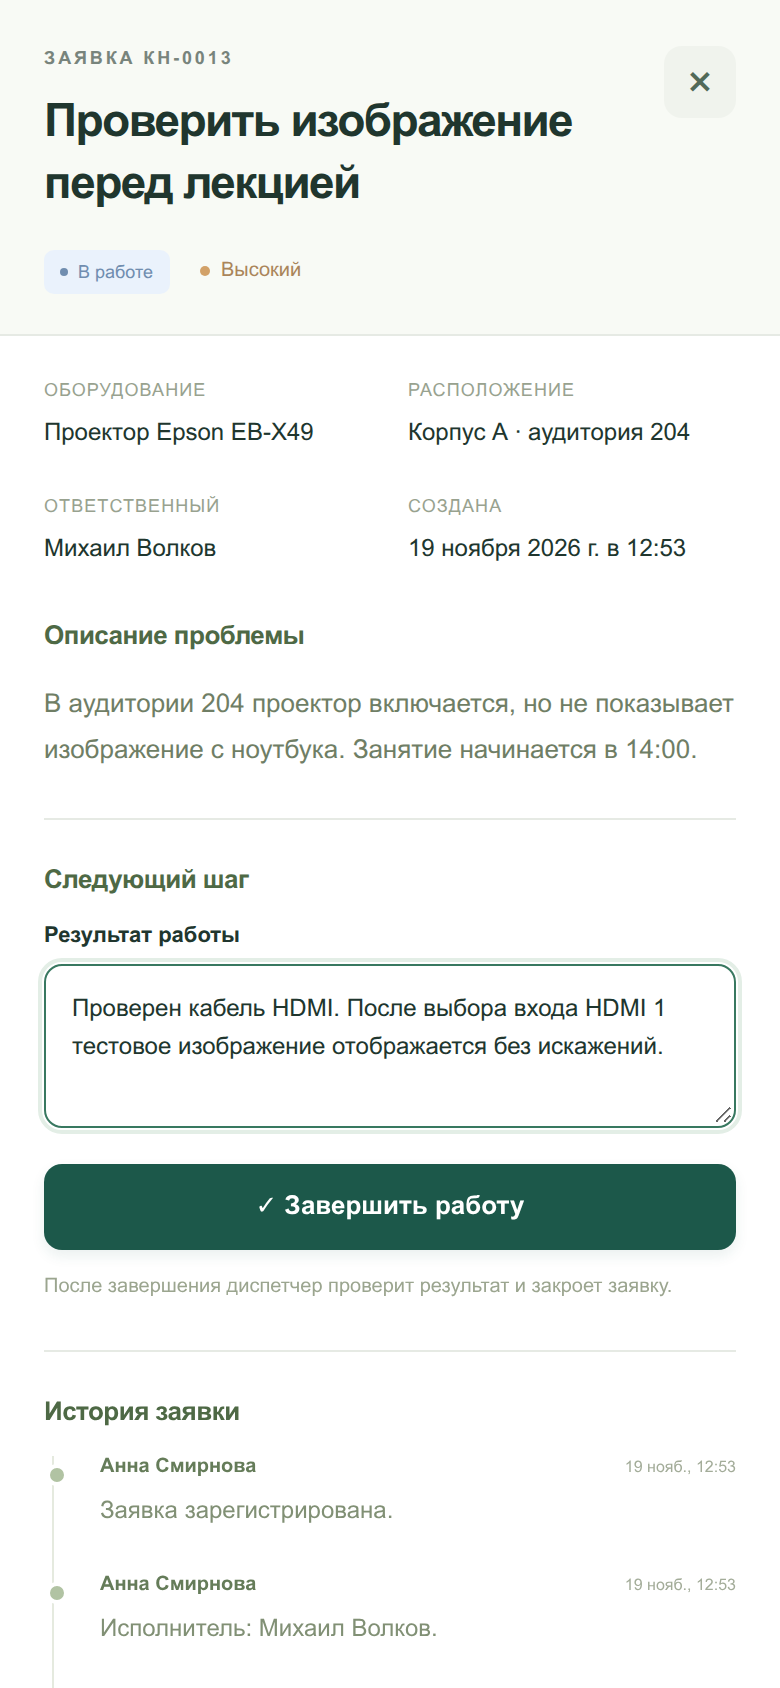
\includegraphics[width=0.51\textwidth,height=0.56\textheight,keepaspectratio]{screens/mobile.png}\caption{Карточка техника в мобильном представлении}\end{figure}

После открытия назначенной заявки техник начинает работу. Этот шаг фиксирует изменение состояния, но не запускает подтверждённый учёт трудозатрат: приложение не измеряет активное время ремонта. Длительность между событиями может включать ожидание деталей или перерыв. Поэтому разность временных отметок нельзя без дополнительных данных выдавать за фактические трудозатраты.

При завершении техник вводит результат: что проверено, что исправлено и остались ли ограничения. Пустая строка, в том числе состоящая только из пробелов, не должна приниматься. Например, результат «заменён кабель питания, выполнена повторная проверка включения» полезнее формального «готово». Программа контролирует наличие текста, но не может гарантировать его техническую достоверность.

При отсутствии связи интерфейс сообщает об ошибке получения или сохранения данных. Офлайн-очередь операций в проекте не реализуется: она потребовала бы правил повторной отправки, разрешения конфликтов и защиты от дублирования. Техник должен видеть, подтверждён ли результат сервером. Сохранение черновика на экране и подтверждение записи в базе — разные состояния.

\section{Обновление данных и устойчивость интерфейса}

Активный клиент периодически запрашивает актуальные данные примерно раз в пять секунд. Такой опрос выбран из-за простоты реализации и достаточности для демонстрационного процесса. Интервал не является гарантией максимальной задержки: к нему добавляются время запроса, нагрузка и особенности фоновых вкладок. Поэтому интерфейс показывает состояние синхронизации, а не обещание «мгновенного» обновления.

Опрос должен обновлять отображаемые сведения, не уничтожая введённый пользователем комментарий. Иначе механизм синхронизации сам становится источником потери работы. Для редактируемой карточки важно сохранить версию, на которой основано действие: подмена её свежим номером без обновления смысла формы сделала бы защиту от конфликтов фиктивной.

Если сервер возвращает конфликт, пользователю следует увидеть сообщение, получить актуальное состояние и повторно оценить действие. Автоматическое повторение прежнего изменения может быть ошибочным. Например, диспетчер собирался сменить исполнителя, пока заявка ожидала начала; после перехода в работу эта операция уже не разрешена. Новая версия не означает, что старое намерение по-прежнему допустимо.

Кнопки изменяющих операций блокируются на время запроса, чтобы уменьшить вероятность повторного нажатия. Однако клиентская блокировка не доказывает однократность доставки: соединение может прерваться после фиксации операции, но до ответа. В таком случае перед повтором требуется обновить карточку. Полноценные ключи идемпотентности для создания заявок остаются возможным дальнейшим улучшением.

\chapter{Проверка, эксплуатация и оценка результата}

\section{Стратегия проверки}

Проверка состоит из нескольких уровней. Серверные тесты обращаются к API с изолированной базой и независимыми клиентами. Они проверяют не внешний вид, а права, переходы, валидацию, конфликт версий и сохранность записей. Проверка браузера оценивает доступность действий, обработку ответов и адаптацию интерфейса. Сценарий на физических устройствах дополнительно проверяет сеть, адрес сервера и работу мобильного браузера.

Эти уровни нельзя подменять друг другом. Успешный серверный тест не доказывает, что на телефоне удобно нажимать кнопку. Скриншот мобильной ширины не доказывает соединение через Wi-Fi. Проверка двух независимых браузерных сеансов подтверждает разделение сессий, но отличается от испытания компьютера и физического телефона. В протоколе следует явно указывать среду каждого наблюдения.

\begingroup\small\singlespacing
\begin{longtable}{>{\raggedright\arraybackslash}p{0.17\textwidth}>{\raggedright\arraybackslash}p{0.39\textwidth}>{\raggedright\arraybackslash}p{0.35\textwidth}}
\caption{Сценарии функциональной проверки}\\
\hline
\textbf{Код} & \textbf{Проверка} & \textbf{Ожидаемый результат} \\ \hline
\endfirsthead
\textbf{Код} & \textbf{Проверка} & \textbf{Ожидаемый результат} \\ \hline
\endhead
Т-01 & Запрос заявок до входа & Отказ без раскрытия списка \\ \hline
Т-02 & Вход с неверным паролем & Сеанс пользователя не создаётся \\ \hline
Т-03 & Создание диспетчером & Запись и событие сохранены \\ \hline
Т-04 & Создание техником & Отказ по полномочиям \\ \hline
Т-05 & Просмотр чужой заявки техником & Содержание не раскрывается \\ \hline
Т-06 & Полный разрешённый цикл & Статусы изменяются последовательно \\ \hline
Т-07 & Завершение без результата & Ошибка, состояние прежнее \\ \hline
Т-08 & Невозможный переход & Ошибка, история не содержит ложного успеха \\ \hline
Т-09 & Два обновления старой версии & Первое сохранено, второе отклонено \\ \hline
Т-10 & Запрос без CSRF-токена & Изменение отклонено \\ \hline
Т-11 & Перезапуск с той же базой & Созданная заявка остаётся доступной \\ \hline
Т-12 & Экспорт потенциальной формулы & Текст не передаётся как активная формула \\ \hline
Т-13 & Потеря сети в браузере & Показана ошибка, нет ложного подтверждения \\ \hline
Т-14 & Узкий экран & Основные действия доступны без широкой таблицы \\ \hline
\end{longtable}
\endgroup

Для каждого отрицательного сценария следует проверять не только код ответа, но и отсутствие нежелательных изменений. Например, отказ технику в закрытии заявки должен оставлять прежний статус и прежнюю версию. Иначе интерфейс покажет ошибку, хотя база уже изменилась. Такая проверка отделяет корректное сообщение от корректного поведения.

\section{Протокол и границы подтверждённых результатов}

Исходный код автоматических проверок находится в каталоге tests. Запуск выполняется командой python -m pytest -q из каталога приложения после установки зависимостей. Окончательный перечень выполненных проверок и их результат следует сопоставлять с сохранённым протоколом проверки поставки. Число тестов не используется как самостоятельная оценка качества: один тест может проверять полный цикл, а несколько простых — только формат ответа.

19 ноября 2026 года выполнены 36 автоматических проверок, все завершились успешно. Среда проверки — Python 3.14.4, Flask 3.1.3, SQLite 3.46.1 и pytest 9.2.0. Из них 33 случая проверяют API, ещё три — создание и чтение резервной копии. В тесте полного цикла заявка создана без исполнителя с версией 1. После назначения, начала работ, передачи результата и приёмки она получила статус «Закрыта» и версию 5. Добавление комментария сохранило версию. В отдельном тесте второй диспетчер попытался изменить уже отредактированную заявку. Сервер вернул HTTP 409. Повторное чтение подтвердило, что сохранились изменения первого диспетчера и только два события — создание и смена приоритета.

В браузерном испытании 19 ноября два независимых сеанса работали через Waitress с отдельной учебной базой. Диспетчер создал заявку № 13 и назначил техника. После обновления очереди техник открыл её, начал работу, добавил комментарий и передал результат. Диспетчер обновил карточку и подтвердил выполнение. Итоговая версия — 5, статус — «Закрыта». В журнале сохранились восемь событий, включая комментарий и результат. Для мобильного сеанса использовано окно 390 × 844 пикселя. Ширина документа составила 390 пикселей, горизонтальная прокрутка не потребовалась. Оба сеанса запускались на одном компьютере. Проверка связи по Wi-Fi между физическим телефоном и компьютером остаётся этапом показа.

Для воспроизведения проверки конкуренции используются два независимых авторизованных клиента, получивших одинаковую версию заявки. Первый изменяет приоритет. Второй пытается сохранить изменение с прежней версией. Ожидается отказ второму запросу и сохранение результата первого. Дополнительно проверяется, что повторная загрузка возвращает увеличенный номер версии. Это предметная проверка защиты от потери обновления, а не замер производительности.

Для проверки разграничения прав создаётся заявка, назначенная первому технику. Второй техник обращается к её карточке напрямую по известному номеру. Отсутствие ссылки в списке недостаточно: прямой запрос тоже должен быть отклонён. Затем назначенный техник начинает работу, завершает её с описанием результата, а диспетчер закрывает. История должна содержать авторов соответствующих действий.

В рамках пояснительной записки не приводятся неподтверждённые показатели экономии времени, скорости отклика или роста производительности труда. Для таких выводов необходимы исходный процесс, сопоставимые задания, условия измерения и достаточное число наблюдений. Здесь оценивается функциональная полнота учебного процесса и воспроизводимость проверок, а не эффективность внедрения в организацию.

\section{Развёртывание и демонстрация на двух устройствах}

Сервер запускается на компьютере с Python и установленными зависимостями проекта. Для демонстрации компьютер и телефон подключаются к одной доверенной сети. В браузере компьютера открывается локальный адрес сервера, а на телефоне — адрес компьютера в этой сети и выбранный порт. Адрес 0.0.0.0 обозначает прослушивание сетевых интерфейсов и не является адресом для ввода в браузере \cite{src3}.

При недоступности страницы с телефона необходимо отдельно проверить сетевой адрес, общую сеть, настройки межсетевого экрана и запрет взаимодействия клиентов в гостевой Wi-Fi-сети. Ошибка соединения до открытия страницы не является ошибкой авторизации приложения. Самовольное отключение защиты компьютера или публикация порта в Интернет для демонстрации не требуются.

Рекомендуемая последовательность показа начинается с диспетчера на компьютере. Он создаёт заявку на выбранное оборудование и назначает техника. На телефоне техник входит под собственной учётной записью, видит новую задачу после обновления, начинает работу, оставляет комментарий и завершает её с результатом. На компьютере диспетчер получает обновлённое состояние, читает журнал и закрывает заявку.

Затем демонстрируется отрицательный сценарий: техник не может создать заявку от имени диспетчера, а устаревшее изменение не перезаписывает свежие данные. Такая часть показа важна, поскольку визуально привлекательный интерфейс не доказывает серверную защиту. После перезапуска сервера повторно открывается созданная заявка, подтверждая постоянство хранения.

Крайний срок предварительного показа по заданию — 25 ноября 2026 года; окончательная сдача предусмотрена в первую неделю декабря. До предварительного показа необходимо выполнить физический сценарий на выбранных устройствах, а после замечаний преподавателя повторить затронутые проверки. Даты определяют организацию работы, но не являются свидетельством уже состоявшейся проверки.

\section{Сопровождение и ограничения}

Резервное копирование реализовано отдельной командой \nolinkurl{scripts/backup.py}. Она открывает исходную базу в режиме чтения, создаёт новый файл средствами SQLite и проверяет целостность полученной копии. При совпадении пути с существующим файлом операция прекращается. Резервная копия должна обеспечивать согласованное состояние SQLite. Для работающей базы предпочтителен штатный механизм резервного копирования, а простое копирование одного файла требует учёта режима журналирования. В учебном сценарии самый понятный вариант — корректно остановить сервер, затем сохранить необходимые файлы данных в защищённом месте. Наличие копии подтверждается пробным восстановлением, а не только её именем.

Обновление программы требует сохранения базы и секрета сеансов вне замены исходных файлов. Изменение схемы данных в будущих версиях потребует миграций. Автоматическая установка новой версии поверх неизвестной базы без проверки совместимости в текущем проекте не рассматривается. Демонстрационную базу нельзя смешивать с реальными обращениями, если работа продолжится в организации.

Основные ограничения: две фиксированные роли, отсутствие офлайн-записи, вложений, уведомлений на закрытом приложении и полноценного администрирования пользователей через интерфейс. Нет интеграции со складом, внешней системой заявок или каталогом сотрудников. Эти возможности не нужны для завершённости выбранного учебного цикла, но должны учитываться при обсуждении практического внедрения.

Направления развития следует выбирать по подтверждённой потребности. Для публичного использования первыми задачами станут HTTPS, управление учётными записями, резервирование и мониторинг. Для большого числа одновременно записывающих пользователей может потребоваться серверная СУБД. Для выездной работы без устойчивой сети — отдельный проект синхронизации с идемпотентностью и разрешением конфликтов. Подключение искусственного интеллекта без такой потребности не улучшает корректность базового процесса.

\clearpage\conclusion

В курсовом проекте разработано приложение «Контур» для управления заявками на обслуживание оборудования. Выбран законченный процесс, в котором диспетчер работает с общей очередью на компьютере, а техник выполняет назначенные задания в мобильном представлении браузера. Общий сервер и база данных связывают действия двух устройств; разные роли определяют доступные сведения и операции.

Спроектированы сущности пользователей, оборудования, заявок и событий. Жизненный цикл разделяет назначение, выполнение и приёмку. Изменение текущего состояния сопровождается записью истории, а контроль версии предотвращает молчаливое сохранение устаревших данных поверх нового состояния. Серверная проверка полномочий обеспечивает соблюдение правил независимо от устройства и способа отправки запроса.

Практическая ценность учебного результата состоит в воспроизводимости: исходный код, демонстрационные данные, проверки и сценарий защиты позволяют проследить полный путь от пользовательского действия до записи в базе. Приложение не требует внешнего облачного сервиса для основного сценария и сохраняет данные между запусками. Адаптивный интерфейс представляет один процесс в формах, подходящих диспетчеру и технику.

Область доказанных выводов ограничена проведёнными проверками, отражёнными в протоколе поставки. Реальное внедрение, экономический эффект, нагрузочная устойчивость и работа на физических устройствах не должны объявляться подтверждёнными без соответствующих испытаний. Дальнейшее развитие связано прежде всего с условиями эксплуатации и реальными потребностями пользователей, а не с добавлением возможностей ради увеличения объёма проекта.

\clearpage\centeredrefname
\phantomsection\addcontentsline{toc}{chapter}{Список использованных источников}
\begin{thebibliography}{99}

\bibitem{src1} Калитвин В. А. tim\_coursework\_template: шаблон оформления курсовой работы в LaTeX. URL: \url{https://github.com/kalitvin/tim_coursework_template} (дата обращения: 09.11.2026).
\bibitem{src2} Pallets Projects. Flask: Quickstart. URL: \url{https://flask.palletsprojects.com/en/stable/quickstart/} (дата обращения: 11.11.2026).
\bibitem{src3} Pallets Projects. Deploying to Production: Waitress. URL: \url{https://flask.palletsprojects.com/en/stable/deploying/waitress/} (дата обращения: 09.11.2026).
\bibitem{src4} SQLite. Transaction. URL: \url{https://www.sqlite.org/lang_transaction.html} (дата обращения: 09.11.2026).
\bibitem{src5} SQLite. SQLite Foreign Key Support. URL: \url{https://www.sqlite.org/foreignkeys.html} (дата обращения: 09.11.2026).
\bibitem{src6} Python Software Foundation. sqlite3 — DB-API 2.0 interface for SQLite databases. URL: \url{https://docs.python.org/3/library/sqlite3.html} (дата обращения: 09.11.2026).
\bibitem{src7} Mozilla. Using the Fetch API. URL: \url{https://developer.mozilla.org/en-US/docs/Web/API/Fetch_API/Using_Fetch} (дата обращения: 09.11.2026).
\bibitem{src8} Mozilla. 409 Conflict. URL: \url{https://developer.mozilla.org/en-US/docs/Web/HTTP/Reference/Status/409} (дата обращения: 09.11.2026).
\bibitem{src9} Mozilla. Using media queries. URL: \url{https://developer.mozilla.org/en-US/docs/Web/CSS/Guides/Media_queries/Using} (дата обращения: 11.11.2026).
\bibitem{src10} OWASP Foundation. Cross-Site Request Forgery Prevention Cheat Sheet. URL: \url{https://cheatsheetseries.owasp.org/cheatsheets/Cross-Site_Request_Forgery_Prevention_Cheat_Sheet.html} (дата обращения: 09.11.2026).
\bibitem{src11} OWASP Foundation. Password Storage Cheat Sheet. URL: \url{https://cheatsheetseries.owasp.org/cheatsheets/Password_Storage_Cheat_Sheet.html} (дата обращения: 11.11.2026).
\bibitem{src12} Pallets Projects. Security Considerations. URL: \url{https://flask.palletsprojects.com/en/stable/web-security/} (дата обращения: 09.11.2026).

\end{thebibliography}
\clearpage\applications

\section*{Приложение А. Контрольный сценарий защиты}
\addcontentsline{toc}{section}{Приложение А. Контрольный сценарий защиты}

\begin{enumerate}
\item Запустить сервер на компьютере, открыть приложение на компьютере и телефоне в одной сети.
\item Войти на компьютере диспетчером, на телефоне — техником. Показать различие доступных действий.
\item Создать заявку с понятным заголовком, описанием, оборудованием и назначенным техником.
\item Дождаться обновления списка на телефоне, открыть задачу и начать работу.
\item Добавить комментарий и завершить работу с конкретным результатом.
\item На компьютере показать результат и журнал, затем закрыть заявку.
\item Показать подготовленный тест конфликта версий и объяснить, почему старое обновление отклоняется.
\item Перезапустить сервер и убедиться, что заявка сохранилась.
\end{enumerate}

\section*{Приложение Б. Различение основных механизмов}
\addcontentsline{toc}{section}{Приложение Б. Различение основных механизмов}

Аутентификация отвечает на вопрос «кто вошёл?». Авторизация определяет, что этому пользователю разрешено. CSRF-защита проверяет допустимость источника изменяющего запроса в контексте сеанса. Валидация проверяет поля и предметные ограничения. Транзакция объединяет связанные изменения. Контроль версии обнаруживает устаревшее намерение клиента. Периодический опрос обновляет представление на экране. Ни один из перечисленных механизмов не заменяет остальные.

\section*{Приложение В. Контрольный пример обработки конфликта}
\addcontentsline{toc}{section}{Приложение В. Контрольный пример обработки конфликта}

В проверке конфликта два диспетчера открывают одну новую заявку. Оба видят обычный приоритет и версию 1. Первый меняет приоритет на высокий и получает версию 2. Второй отправляет низкий приоритет и ожидаемую версию 1. Сервер отвечает HTTP 409. После повторного открытия оба диспетчера видят высокий приоритет. В журнале остаются регистрация и одна смена приоритета. Пользователь может выбрать низкий приоритет повторно, уже учитывая изменение коллеги.
\end{document}
